\chapter{実験}
\label{chap:exeperiment}


\section{実験の目的}
\label{sec:purpose}

節\ref{sec:curb}で述べたような、電力ー実行時間曲線の違いによって生じる電力を増減させたときの実行時間の変動幅の違いを利用した性能向上手法は今のところ先行研究が存在しない。そのため、本実験において蓄電池を用いて理想的な電力融通を行うことができた場合にどれほどの効果があるのかを見積もることが第一の目的である。また同じく節\ref{sec:curb}で述べたように、プロセッサの周波数が離散的な値しか取ることができないことによって生じる余剰電力を利用した効果もあると予想されるため、その効果もできる限り個別に評価する。これが第二の目的である。

以下、これら二つの目的を達成するための実験方法及びその結果・考察について述べる。


\section{実験方法}
\label{sec:method}

本手法を用いた性能向上を実現するためには以下の3つの段階を踏む必要がある。

\begin{enumerate}
\item ユーザがアプリケーションのソースコードに埋め込んだフェーズ区切り文を読み取り、アプリケーションを分割する。
\item 分割されたフェーズそれぞれについて電力ー実行時間曲線を求める
\item 分割されたフェーズに対する電力融通問題を解く
\end{enumerate}

まず、1段階目について述べる。実際に節\ref{sec:phase2}のように書かれたソースコードからフェーズ区切り文を読み取るのはコンパイラレベルでの実装が必要となり困難である。そのため、本実験ではそのフェーズに入ったもしくは出た時刻をログとして出力する自作関数をソースコードに埋め込むことによって、その代わりとした。また、今回実験に利用したアプリケーションは自作のものではないので、ソースコードを読んでどの部分がフェーズの区切りであるかを完全に知ることは困難であった。そこで簡単のため、並列処理部分と逐次処理部分のみをソースコードから判別してフェーズ分割を行った。そして、プロセッサの取りうる全てのDVFSパターンについてアプリケーションを実行し、ログファイルを得た。ただし表\ref{tbl:parsec}に示したアプリケーションのうち、QT Clusteringのみは並列実行の中に2つのフェーズがあったため、全体で並列処理1・並列処理2・逐次処理の3フェーズに分割した。

次に2段階目である。ここでは1段階目で得たログファイルから、それぞれのフェーズについて全てのDVFSパターンにおける平均電力と実行時間を得ることができる。それを用いてそれぞれのフェーズの電力ー実行時間曲線を計算した。ただし実際にはDVFSパターンは有限であるので、電力ー実行時間曲線は図\ref{fig:discrete_power_time}のようになった。

\begin{figure}[t]
 \begin{center}
  \includegraphics[width=110mm]{discrete_power_time.eps}
 \end{center}
 \caption{離散的な周波数しか取れない場合の電力ー実行時間曲線}
 \label{fig:discrete_power_time}
\end{figure}

最後に3段階目は、節\ref{sec:algorithm}で述べたように得られた電力ー実行時間曲線から総当たりで最適なDVFS設定値を見つけた。

また節\ref{sec:purpose}で述べたように、本実験の目的は電力ー実行時間曲線の違いを利用した性能向上と、プロセッサの動作周波数が離散的であることを利用した性能向上のそれぞれを評価することである。ここまでの実験方法では両者の影響が入り交じった結果のみしか得られない。そこで、2段階目で得られた電力ー実行時間グラフを式\ref{asm:model}に合うように補間することによって、連続な電力ー実行時間グラフを得た(図\ref{fig:continuous_power_time})。ただし完全に連続であると電力融通問題を総当たりで解くことができなくなるため、実際にはある程度の細かい間隔で補間することで連続的な曲線への近似とした。そして、3段階目では同様に総当たりで最適なDVFSの設定値を見つけ、周波数が離散的な場合の結果と比較することによって、電力ー実行時間曲線の違いによる効果とプロセッサが離散的であることによって生じる余剰電力による効果のそれぞれを見積もった。

\begin{figure}[t]
 \begin{center}
  \includegraphics[width=110mm]{continuous_power_time.eps}
 \end{center}
 \caption{連続補間した場合の電力ー実行時間曲線}
 \label{fig:continuous_power_time}
\end{figure}

用いたベンチマークアプリケーションは表\ref{tbl:parsec}の通りである。CPU並列のアプリケーションではCPUの電力のみ、GPU並列のアプリケーションであればGPUの電力のみを測定した。

\begin{table}[t]
\begin{center}\begin{tabular}{|c|c|c|}
\hline ワークロード名 & & 説明 \\
\hline PARSEC Canneal & CPU並列 & \shortstack{SAアルゴリズムを用いてルーティングコストが\\最小となるchipを設計する. }\\
\hline PARSEC Stream Cluster & CPU並列 & \shortstack{ストリーミングされる点列の\\オンラインクラスタリングを行う. }\\
\hline Rodinia mummergpu & GPU並列 & 深さ優先探索によりDNA塩基配列を求める\\
\hline SHOC QT Clustering & GPU並列 & \shortstack{クラスタメンバ間の相関が指定されたカットオフ値より\\高いことを保証するクラスタリング}\\
\hline \end{tabular} \caption{使用したベンチマークアプリケーションの詳細}\label{tbl:parsec}
\end{center}
\end{table}



\section{結果}
\label{sec:result}

それぞれのアプリケーションの電力ー実行時間曲線を図\ref{fig:canneal_power_time}、\ref{fig:streamcluster_power_time}、\ref{fig:mummergpu_power_time}、\ref{fig:qtclustering_power_time}に、スピードアップ曲線を図\ref{fig:canneal_speedup}、\ref{fig:streamcluster_speedup}、\ref{fig:mummergpu_speedup}、\ref{fig:qtclustering_speedup}に示す。ただし、スピードアップは以下のように定義される。

\begin{eqnarray}
スピードアップ =  1 - \frac{{\rm UPS}ありの場合のアプリケーション全体の実行時間}{{\rm UPS}なしの場合のアプリケーション全体の実行時間}
\end{eqnarray}


Cannealの電力ー実行時間グラフは並列処理と逐次処理の電力消費の違いをよく表しており、並列処理の方が逐次処理より大きい電力を消費していることが分かる。Stream Clusterも同様の傾向は見て取れるが、Cannealとは違って逐次処理部分の実行時間が非常に短いことが特徴である。mummergpuのグラフを見ると、どのDVFS設定においても逐次処理部分の実行時間が変わらないことが分かる。これは節\ref{sec:method}で述べたようにGPU並列アプリケーションはGPUの電圧のみを測定しているため、CPUで演算をしている逐次処理部分はの実行時間はGPUの周波数に影響を受けないためである。QT Clusteringでは3つのフェーズがあり、mummergpu同様に逐次処理部分はDVFSの設定によらずほぼ同じ実行時間になっている。

次にスピードアップのグラフについてであるが、全体的に離散的な周波数しか取れない場合の方が、連続的に周波数を変化できる場合に比べて効果は大きかった。また離散的な場合は電力制約ごとにスピードアップの変動が大きく、大きくスピードアップする場合もあれば全くスピードアップしない場合もある。連続の場合では、離散的な場合のようにスピードアップの値が大きく変動することはなかったが、やはり電力制約に応じてある程度の変動は見て取れる。

\begin{figure}[t]
 \begin{center}
  \includegraphics[width=110mm]{canneal_power_time.eps}
 \end{center}
 \caption{Canneal 電力ー実行時間曲線}
 \label{fig:canneal_power_time}
\end{figure}

\begin{figure}[t]
 \begin{center}
  \includegraphics[width=110mm]{streamcluster_power_time.eps}
 \end{center}
 \caption{Stream Cluster 電力ー実行時間曲線}
 \label{fig:streamcluster_power_time}
\end{figure}

\begin{figure}[t]
 \begin{center}
  \includegraphics[width=110mm]{mummergpu_power_time.eps}
 \end{center}
 \caption{mummergpu 電力ー実行時間曲線}
 \label{fig:mummergpu_power_time}
\end{figure}

\begin{figure}[t]
 \begin{center}
  \includegraphics[width=110mm]{qtc_power_time.eps}
 \end{center}
 \caption{QT Clustering 電力ー実行時間曲線}
 \label{fig:qtclustering_power_time}
\end{figure}

\begin{figure}[t]
 \begin{center}
  \includegraphics[width=110mm]{canneal_speedup.eps}
 \end{center}
 \caption{Canneal スピードアップ曲線}
 \label{fig:canneal_speedup}
\end{figure}

\begin{figure}[t]
 \begin{center}
  \includegraphics[width=110mm]{streamcluster_speedup.eps}
 \end{center}
 \caption{Stream Cluster スピードアップ曲線}
 \label{fig:streamcluster_speedup}
\end{figure}

\begin{figure}[t]
 \begin{center}
  \includegraphics[width=110mm]{mummergpu_speedup.eps}
 \end{center}
 \caption{mummergpu スピードアップ曲線}
 \label{fig:mummergpu_speedup}
\end{figure}

\begin{figure}[t]
 \begin{center}
  \includegraphics[width=110mm]{qtc_speedup.eps}
 \end{center}
 \caption{QT Clustering スピードアップ曲線}
 \label{fig:qtclustering_speedup}
\end{figure}


\section{考察}
\label{sec:discussion}

4つのアプリケーションの中で、Stream Clusterのみは蓄電池を用いた電力融通にスピードアップがとても小さかった。これは、逐次処理部分の実行時間が並列処理部分の実行時間と比べて非常に短かったため、蓄電池が充放電する時間がほとんどなく、電力融通を上手く行うことができなかったためであると考えられる。しかし、離散の場合には電力制約によってはところどころ針が立ったように大きくスピードアップしている部分がある。これはもう少し電力制約が大きくなればもう一つ上の周波数に上げることができる、という状況で起こるものである。逐次処理でわずかに蓄えたエネルギを並列処理部分に融通することで、周波数を一段階上げることができたのである。周波数が連続的に変えられる場合には、周波数を数段階上げる程度では大した時間短縮にはならないため、このようなことは起こらない。

全てのアプリケーションを通して、離散的な周波数しか取れない場合の方が連続的に周波数を変化させられる場合に比べて効果は大きかった。これは節\ref{sec:curb}で述べたように、周波数が離散的であるために生じる余剰電力を蓄電池を用いて融通することによる性能向上効果のためであると考えられる。

全体的に、離散的な周波数しか取れない場合には電力制約ごとにスピードアップの値が大きく異なる。これまでに述べたように離散的であると余剰電力は多く生じるのだが、周波数を一段階上げるために必要なエネルギ融通量も大きくなる。また、周波数を一段階上げたときに短縮される実行時間も大きい。そのため、上手く周波数を上げられるような電力制約の場合は大きくスピードアップする一方で、逆に周波数を上手く上げられないような電力制約ではほとんどないし全くスピードアップさせることができないのである。

最後に、連続的に周波数が変更できる場合にどのような周波数が最適解となっているかについて考察する。









